\section{Introduction}

ImageJ macro is a useful tool to automate image processing and analysis. In this tutorial, we learn how to write a macro for analyzing intensity dynamics from a time lapse sequence. 

Analysis is done by processing a two-channel image stack, a time lapse sequence of the process of NPC protein relocalizing from cytoplasm to the nuclear membrane\footnote{Courtesy of Andreas Boni}. Two images shown in figure \ref{fig:NucStrategy}  are from the first and the last time points of the movie\footnote{The original 4D hyperstack file is NPC1.tif. You could load the file via CourseModule plugin.}.

Compare these images carefully. You might recognize that the green signal in the periphery of nuclei (red) is stronger in the second image. We want to write a macro to compare this difference in a quantitative way. The processing involves two steps: We first segment the nucleus in a first (histone) channel. Second, we use that segmented nucleus rim as a mask to measure the intensity changes in the second channel. 

\begin{figure}[htbp]
 \centering
 \subfloat[Time point 1]{\label{fig:NucTimePoint1}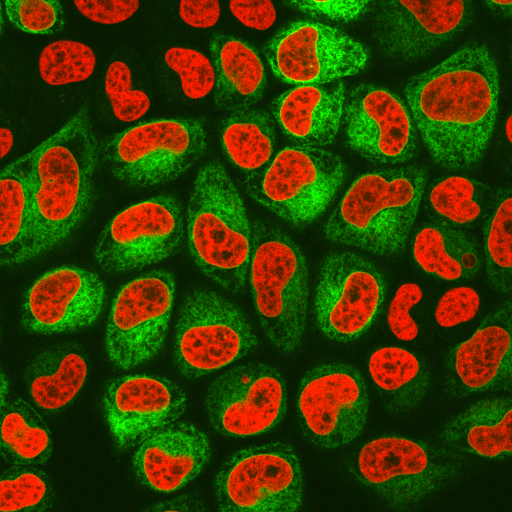
\includegraphics[width = 0.45\textwidth]{fig/NPC_T01.png}} 
 \quad
 \subfloat[Time point 15]{\label{fig:NucTimePoint15}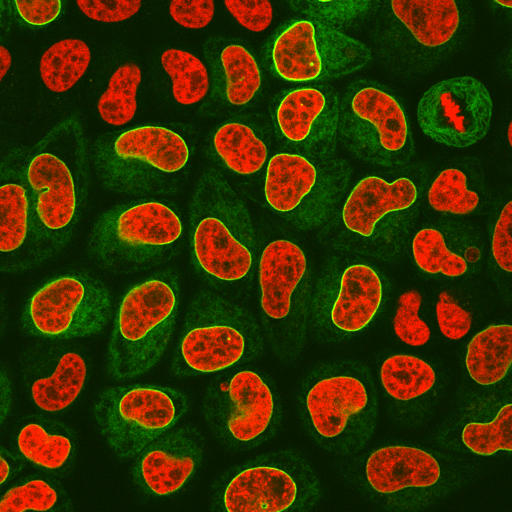
\includegraphics[width = 0.45\textwidth]{fig/NPC_T15.png}} \\
 \caption{NPC localization difference at two time points: More NPC in nucleus periphery. }
 \label{fig:NucStrategy}
\end{figure}

This tutorial could be a good guide line for those interested in segmenting the edge (perimeter) of biological object, by learning a typical usage of morphological processing for segmenting object boundaries. 

\section{Measurement of Nucleus Periphery Intensity}

To simplify the development, we limit our work on single nucleus. Load the image stack \textbf{NPCsingleCell.tif}. This is a hyperstack sequence. Slide the scroll bar at the bottom back-and-forth to watch the process of intensity changes. Histone signal is more or less constant, but the NPC signal (labeled in green) shows strong accumulation to the nuclear membrane. To quantify this process, we measure the intensity changes in the nuclear rim over time.

For this we first need to identify where the nuclear rim is (``segmentation''). We then have a mask for the rim. Using this mask we measure the changes in intensity over time. We first write a macro for the nucleus rim segmentation. 

\subsection{Segmentation of Nucleus Rim}

To segment the nucleus rim, we take following steps. It's rather long but if you once write a macro everything could be done by running the macro by a single click. 

\begin{enumerate}
  \item Split channels (fig. \ref{fig:originalNucleus})
    \item Blur the image (fig. \ref{fig:BlurredNucleus})
    \item Binarize the image by intensity thresholding (fig. \ref{fig:BInarizedNucleus})
    \item Remove other Nucleus
    \item Duplicate the image
    \begin{enumerate}
        \item Erode one of them (fig. \ref{fig:erodedBinary})

        \item Dilate one of them (fig. \ref{fig:dilatedBinary})

    \end{enumerate}
    \item Subtract the eroded from the dilated (fig. \ref{fig:NucleusRim})

\end{enumerate}

\begin{figure}[h!]
 \centering
 \subfloat[Original Nucleus Image]{\label{fig:originalNucleus}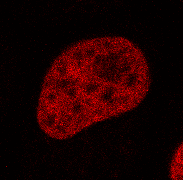
\includegraphics[width = 0.30\textwidth]{fig/OriginalNuc.png}} 
 \quad
 \subfloat[Blurred Nulcleus Image]{\label{fig:BlurredNucleus}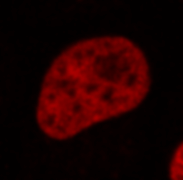
\includegraphics[width = 0.30\textwidth]{fig/BlurredNuc.png}}
 \quad
 \subfloat[Binarized image, after thresholding.]{\label{fig:BInarizedNucleus}
\includegraphics[width = 0.30\textwidth]{fig/ConvertedMask.png}} \\
 \subfloat[Dilated Binary Image]{\label{fig:dilatedBinary}
\includegraphics[width = 0.30\textwidth]{fig/dilated.png}}
 \quad
 \subfloat[Eroded Binary Image]{\label{fig:erodedBinary}
\includegraphics[width = 0.30\textwidth]{fig/eroded.png}}
 \quad
 \subfloat[Subtraction Result, the rim.]{\label{fig:NucleusRim}
\includegraphics[width = 0.30\textwidth]{fig/NucRim.png}}
 \caption{Strategy of measurement.}
 \label{fig:nucsegProc}
\end{figure}


In the following we record most of the commands using the Command Recorder (\ijmenu{[Plugins > Macros > Record\ldots]}). I recommend you NOT to startup the command recorder from the beginning. Follow the protocol first using GUI. Record commands only when you become sure with what you are doing. When you use the command recorder, be sure that ``Macro'' is selected in the ``Record:'' drop down menu at the top-left corner of the recorder.

\subsubsection{Splitting Channels}

To split the multichannel image stack from the GUI menu, do \ilcom{[Image > Color > Split Channels]}. In the Recorder, you would see the following command in the history. 
\begin{lstlisting}[numbers=none]
run("Split Channels");
\end{lstlisting}

\ilcom{run} function is the most frequently used build-in macro function. 

\fbox{
\parbox[b][15em][c]{0.80\textwidth}{
  \textbf{run("command"[, "options"])}
  Executes an ImageJ menu command. The optional second argument contains values that are automatically entered into dialog boxes (must be GenericDialog or OpenDialog). Use the Command Recorder (Plugins>Macros>Record) to generate run() function calls. Use string concatenation to pass a variable as an argument. With ImageJ 1.43 and later, variables can be passed without using string concatenation by adding "\&" to the variable name.
}}

The run function takes a menu item as the first argument, and optional values (values you fill in in dialog for many of the functions) in the second argument. In case of channel splitting, there is no option so the second argument is ignored. 

We now want to work on the nucleus image. Activate (Click a window to bring up to the top) Channel 2 (red, nucleus image).

In the recorder, the function \ilcom{selectWindow("C1-NPCsingleNucleus.tif");} appears. 

\fbox{
\parbox[b][3em][c]{0.80\textwidth}{
  \textbf{selectWindow("name")}\\
Activates the window with the title "name".
}
}

This function takes a title of a window as an argument and activates that window. When we used mouse to activate the nucleas channel stack, we did it manually by visually recognizing the name of the window. On the other hand, we want to figure out the name of the windows of each individual channles by some commands within macro so we could choose them using ``selectWindow''command after channel-splitting.  

Standard behavior of ``Split Channel'' command is that it automatically names the resulting stacks of individual channels by appending ``C1-'' or ``C2-'' or ``C3'' in front of the original image title. We can construct these names if we knew the original image title. For this we use the command \ilcom{getTitle()} which returns the image title as a string. 

\fbox{
\parbox[b][3em][c]{0.80\textwidth}{
\textbf{getTitle()}\\
Returns the title of the current image.
}
}

Here is the code to activate the nucleus channel automatically after the splitting. More importantly, we also acquire ``image ID''. This will be explained later.  

\begin{lstlisting}
orgtitle = getTitle();
run("Split Channels");
c1name = "C1-" + orgtitle;
c2name = "C2-" + orgtitle;
selectWindow(c1name);
c1id = getImageID();
selectWindow(c2name);
c2id = getImageID();
\end{lstlisting}

\textbf{Details:} 
\begin{itemize}
\item The first line grabs the window title as ``orgtitle''. 
\item The second line splits the stacks to individual stacks for each channel.
\item 3rd and 4th lines construct the window name of each channel stacks. 
\item 5th line activates the channel 1 stack. 
\item 6th line acquires the image ID of channel 1 stack. 
\item 7th line activates the channel 2 stack. 
\item 8th line acquires the image ID of channel 2 stack. 
\end{itemize}


In lines 6 and 7, we acquire image IDs. Here is some more explanation about this: Each window has a unique ID number. To get this ID number from each image we use the command \ilcom{getImageID()}.

\begin{indentCom}
\fbox{
\parbox[b][8em][c]{0.80\textwidth}{
\textbf{getImageID()}\\
Returns the unique ID (a negative number) of the active image. Use the selectImage(id), isOpen(id) and isActive(id) functions to activate an image or to determine if it is open or active.
}
}
\end{indentCom}

A window can be activated by \ilcom{selectWindow} using its window title, but this could have a problem if there is another window with same name. Image ID has less problem since it is uniquly given to each window. To select a window using image ID, we use ``selectImage(ID)'' command.

\begin{indentCom}
\fbox{
\parbox[b][8em][c]{0.80\textwidth}{
\textbf{selectImage(id)}\\
Activates the image with the specified ID (a negative number). If id is greater than zero, activates the idth image listed in the Window menu. The id can also be an image title (a string).
}
}

\end{indentCom}

We acquire image IDs just after the splitting for future use, when we want to specify the image we want to work on. 

\begin{indentexercise}{1}
Test the code below and run it on different windows. Confirm that each window has different ID number. 
%\begin{lstlisting}[numbers=none]
\begin{lstlisting}
id = getImageID();
print( id );
name = getTitle();
print( name );
\end{lstlisting}
\end{indentexercise}


\subsubsection{Isolating Rim Mask}

Now we start working on the detection of nucleus rim. Save the channel splitting macro. When you name the file, add an extension ``.ijm'', as this indicates that the file is an ImageJ macro. 

Create a new tab in the script editor by \ilcom{[File > New]}. We work in a new file only to create a macro for the detection of nucleus rim. We assemble them later. 

Following is the step-by-step procedure. Try first from the GUI (mouse and the menu bar!). Then reopen the macro recorder to record history of commands. I recommend you to do so because the trial with GUI let you understand what is going on.  

\begin{enumerate}
  \item Gaussian Blur
  \begin{itemize}
    \item \ijmenu{[Process > Filter > Gaussian Blur]}, sigma = 1.5, Do Stack.
    \item Blurring image slightly removes noise. Better results for the thresholding below.  
  \end{itemize}
  \item Find Threshold
  \begin{itemize}
    \item \ijmenu{[Image > Adjust > Threshold]},  Otsu method
    \item This simply changes the LUT, not the data. 
  \end{itemize}
  \item Apply Threshold: Click 'Apply'
  \begin{itemize}
    \item Changes the data to black and white according to the above Otsu based threshold value. 
  \end{itemize}
  \item Find Threshold again (Otsu method)
  \begin{itemize}
    \item We do this again for selecting nucleus for the ``AnalyzeParticle'' in the following.
  \end{itemize}
  \item Analyze Particles
  \begin{itemize}
    \item \ijmenu{[Analyze > Analyze Particles]}
    \item Options::
    \begin{itemize}
      \item Size: 800-Infinity
      \item Check ``Pixle Units''
      \item Circularity: default (0 - 1.0)
      \item Show: Mask
      \item Check Display Results, Clear results, Exclude on edges, Include holes. 
    \end{itemize}
    \item We use AnalyzeParticle as a filter for segmented object. In our case, this filtering removes nucleus touching the edge of image. This way of usage is also effective in removing small none-nucleus signals. 
  \end{itemize}
  \item Use the "Mask" output. Invert LUT
  \begin{itemize}
    \item \ijmenu{[Image > Look-up Table > Invert LUT]}
  \end{itemize}
  \item Duplicate Stack, because we erode one and dilate the other.
  \begin{itemize}
    \item \ijmenu{[Image > Duplicate]}
    \item Set Iterations \ijmenu{ [Process > Binary > Options]}
    \begin{itemize}
      \item iterations 2 or 3
      \item dark background
    \end{itemize}
    \item Original: Dilate \ijmenu{[Process > Binary > Dilate]}
    \begin{itemize}
      \item This increases the edge of nucleus by 2 or 3 pixels. 
    \end{itemize}
    \item Duplicate: Erode \ijmenu{[Process > Binary > Erode]}
    \begin{itemize}
      \item This decreases the edge of nucleus by 2 or 3 pixels. 
    \end{itemize}
  \end{itemize}
  \item Image Subtraction
  \begin{itemize}
    \item \ijmenu{[Process > Image Calculator]}
    \item keep original, difference of Dilated and Eroded.
    \begin{itemize}
      \item Leaves a band of 4 or 6 pixels at the edge of nucleus. 
    \end{itemize} 
  \end{itemize}
\end{enumerate}

If you could successfully do the processing and its macro recording, check the results in the recorder. Below is an example of the direct output from the recorder. 

\lstinputlisting{code/code_recordNucSeg.ijm}

This already is a macro that runs properly. But there is a problem: the code should be improved to increase the generality of code. Not general, because for example if you see the line 1, the command is 

\ilcom{selectWindow("C1-NPCsingleNucleus.tif");}. 


As explained in above already, this is a very specific command that activates only a window with specific title. We rather want to use ImageID. Since we know the ImageID of nucleus channel already (which we acquired after splitting the original image), we could use that ID number to activate the window we want to work on. For now we assume that the nucleus channel stack is at the top and replace the first line with \ilcom{getImageID()} command. 

Using image IDs, we could upgrade the code as follows.  If you go through the code towards bottom, we should also replace selectWindow function to selectImage funciton in line 12 and 15.


\lstinputlisting[morekeywords={*, getImageID, selectImage, orgID, dilateID, erodeID}]{code/code_recordNucSegV2.ijm}

Here is the explanation of what was done. 
\begin{itemize}
  \item line 1: The first line is replaced with getImageID() command. 
  \item line 10: getImageID() command inserted for a new image created by Analyze Particle command (in line 9). The new image is the mask that is eliminated with edge-touching nucleus. 
  \item line 13: getImageID() command inserted for the duplicated image. 
  \item line 15: selectWindow command in line 14 is commented out and replaced by selectImage command. 
  \item line 19: similarly, selectWindow command is replaced by selectImage command. 
  \item line 22: Because we now have imageIDs of both dilated and eroded images, we could replace the specific names of the images to imageID. Compare the line 21 (commented out) and the line 22. 
\end{itemize}

We are now almost done with the generalization of the code, but there still is a line that is not general. See line 12. This line using \ilcom{run} command to duplicate the stack.

The command looks like this:

\ilcom{run("Duplicate...", "title=[Mask of C1-NPCsingleNucleus-1.tif] duplicate range=1-15");}

The first argument ``Duplicate\ldots'' is the menu item at \ijmenu{[Image > Duplicate\ldots]}. The second argument contains multiple optional values you choose in GUI. The first is the title of the image that will be duplicated. In the above case, a long name is given to the duplicated image. Square brackets surrounding the title is for suppressing problem with spaces in the name, because spaces are the separator for the options in the second argument. ``duplicate'' is a keyword for a checkbox in the duplication dialog, whether to duplicate multiple frames in a stack or just a single currently shown frame. The third option is a frame range, which defines the range of frames to be duplicated. Since we want to duplicate all frames, the range is set to 1-15, from first frame to the last 15th frame.

There are two parameters in this command that are not flexible enough for various images. First is the title. We could have a more general name for the duplicated image. The second is the frame range.  The duplication of full stack should be achieved for stacks with any number of frame, not limited to 15 frames stacks. 

We can construct the option string (the second argument) as follows to solve these problems. 

\ilcom{options = "title = dup.tif duplicate range=1-" + nSlices}

\ilcom{nSlices} is a macro function that returns the number of frames or slices in the current stack. 

We can now replace the second argument for image duplication by this new variable "options". 

\ilcom{run("Duplicate...", options);}

\begin{indentexercise}{2}
Create a new script tab and write the following code. Run it with several stacks with different frame numbers and confirm that this short macro successfully duplicate stacks with different slize numbers. 
\begin{lstlisting}
print(nSlices);
options = "title=dup.tif duplicate range=1-” + nSlices;
print(options);
\end{lstlisting}
\end{indentexercise}

Below is the upgraded code. All the lines previously commented out were removed, and line 10 is now inserted for preparing options for the Duplicate command. 

\lstinputlisting{code/code_recordNucSegV3.ijm}

We now have a macro that segments nucleus rim. Save this macro.

We move on to do the stack measurement. 

\subsection{Intensity Measurement using Mask}

Using the isolated nucleus rim image, we could specify the region where we measure the intensity in the NPC channel (called ``redirection'' in ImageJ). We first do this in GUI: Open the rim binary image (if you closed it already, run the macro to regenerate it!) and the NPC image. 

Our aim is to write a macro that does the full processing starting from original two channel stack. But just for the reason to develop in modular way and assemble afterwards, we use the rim-segmented stack and the original NPC stack as source images to measure the NPC intensity at the nucleus rim. We combine the segmentation part afterwords. For this reason we merge rim-segmented stack and the NPC stack to create a mock-multichannel stack.  

\begin{figure}[h!]
\begin{center}
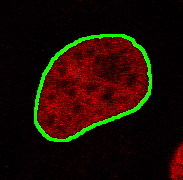
\includegraphics[scale=1.0]{fig/NucRimMerged.png}
\caption{Segmented rim and NPC channel merged.}
\label{fig:NucRimMerged}
\end{center}
\end{figure}

Let's merge two stacks to generate a two channel image stack. 

\ilcom{[Image > Color > Merge Channels\ldots]}

Assign NPT channel to be green, and nucleus (histone) channel to be red. We now have an image stack that looks like figure \ref{fig:NucRimMerged}.

\begin{figure}[h!]
\begin{center}
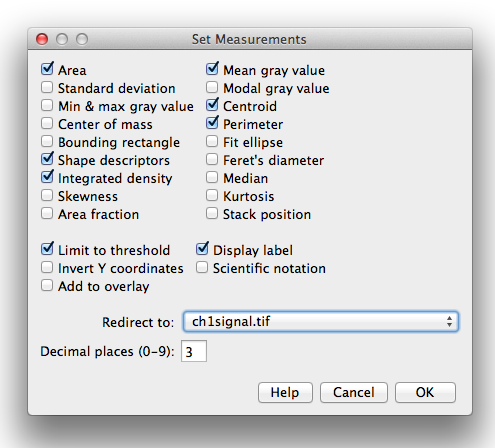
\includegraphics[scale=0.5]{fig/SetMeasurementsRedirect.png}
\caption{Measurement Setting with redirection.}
\label{fig:MeasSettingRedirect}
\end{center}
\end{figure}


We do the following. 

\begin{enumerate}
  \item \ijmenu{[Image > Color > Split Channels\ldots]}
  \item \ijmenu{[Analysis > Set Measurements\ldots]}
  \begin{itemize}
    \item Set the redirection to NPC stack. You will see a dialog window with many check boxes (\ref{fig:MeasSettingRedirect}). Among the parameters to be measured, check at least Area, Mean Gray Value and Integrated Intensity. Integrated Intensity is the sum of all pixel values. A very important setting is "Redirect to". By default ``None'' is selected in the drop-down menu, but here you select the NPC channel image.
    \item Redirection of measurement means that the measured values are not from currently active image, but from another image specified in the setting window. In our case, we want to specify the region for measurement using rim image and do the measurement in the other image (NPC signal). 
  \end{itemize}
  \item Activate the rim image and do \ijmenu{[Edit > Selection > Create Selection]}
  \begin{itemize}
    \item This selects the background, not the rim. 
  \end{itemize}
  \item \ijmenu{[Edit > Selection > make Inverse]}
  \begin{itemize}
    \item Inverting the selection, now we are selecting the nucleus rim. 
  \end{itemize}
  \item \ijmenu{[Analyze > Measure]}
\end{enumerate}

Selection of the rim should look like figure \ref{fig_RoiNucRim}.

\begin{figure}[h!]
\begin{center}
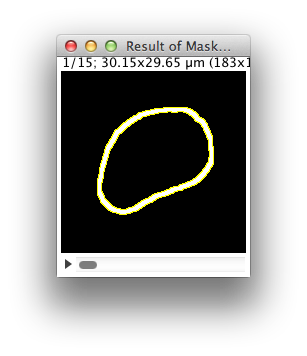
\includegraphics[scale=0.8]{fig/ROIselectionNucRim.png}
\caption{ROI selection of nucleus rim. }
\label{fig_RoiNucRim}
\end{center}
\end{figure}

You will then see results in the Results table like in figure \ref{fig_NucRimMeasureResults}

\begin{figure}[h!]
\begin{center}
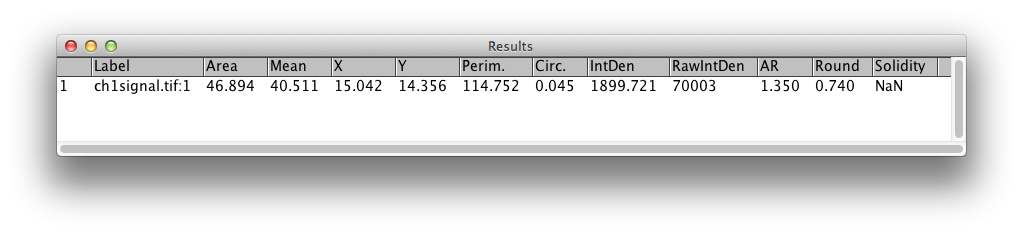
\includegraphics[width=0.95\textwidth]{fig/MeasurementResults.png}
\caption{Results output.}
\label{fig_NucRimMeasureResults}
\end{center}
\end{figure}

If you record these procedures in the macro recorder, it should be pretty simple like shown below. Create a new tab in the Script Editor and copy \& paste (or if not possibe, click ``create'' button in the Recorder).

\begin{lstlisting}
run("Split Channels");
run("Set Measurements...", "area mean centroid perimeter shape integrated limit display redirect=C2-Composite decimal=3");
selectWindow("C1-Composite");
run("Create Selection");
run("Make Inverse");
run("Measure");
\end{lstlisting}

In the 1st line, we split the multichannel stack to do processing individually. Resulting image window names are specific to the source image name we used for the recording and this specific name is used in the second and the third line:  We have encounterd such non-general codes already and we know how to deal with this - construct image window names after splitting and also acquire their image IDs. We could use the code we wrote already in the section ``Splitting Channels''. 

\begin{lstlisting}[morekeywords={*, c1, c2, opt, getTitle}]
orgName = getTitle();
run("Split Channels");
c1 = "C1-" + orgName;
c2 = "C2-" + orgName;
selectWindow(c1name);
c1id = getImageID();
selectWindow(c2name);
c2id = getImageID();
opt = "area mean centroid perimeter shape integrated limit display redirect=" + c1 + " decimal=3";
run("Set Measurements...", opt);
selectWindow( c2 );
run("Create Selection");
run("Make Inverse");
run("Measure");
\end{lstlisting}

The upgraded code first captures the title of the multi-channel image. This will be used in the third and fourth lines. Then the channels are separated into two stacks. Since we know the rule of how the resulting image stack names are, we construct titles each for channel 1 and channel 2. We then acquire image IDs. Finally,  we compose the argument for the ``Set Measurement'' and generalize the window name in ``setWindow'' line. 

\begin{indentexercise}{1}
Merge rim and NPC image stacks and test the code. 
\end{indentexercise}

\subsubsection{Adding for-loop}

As you may have already realized, the code above measures only one frame. To measure the intensity changes over time, we need to add some looping to do the measurement. We already did this in thefirst section so you already know how it works. We just need to modify that code and is very simple.

\lstinputlisting[morekeywords={*, for, nSlices, setSlice}]{code/code_redirectedMeasurement.ijm}

\begin{indentexercise}{2}
Merge rim and NPC image stacks and test the code to see if it measures intensity in the nuclear rim over time frames. 
\end{indentexercise}

\subsubsection{Integrating Segmentation and Measurements}

Finally, we can integrate segmentation macro and intensity measurement macro. With the last code, we used  two-channel stack with rim mask and the NCP signal. All we need to do is to insert the segmentation part between line 4 and line 5 since if we use the original multi-channel stack, c2 will be the name of unprocessed histone stack. 

A simple way to do this is to convert the segmentation macro to a use-defined function. Like all the macro commands that you see in the ImageJ macro function reference list, you could create one by your self. To do so, we first learn with a very simple function. 

If we have a macro like below:

\begin{lstlisting}
a = 10;
b = 20;
c = a + b + a * b ;
print c;
\end{lstlisting}

It probably is evident for you that there will be an output in the log window "230". We could make a function that does the calculation in line 3 in the following way.

\begin{lstlisting}[morekeywords={*, function, return}]
a = 10;
b = 20;
c = calc1(a, b);
print c;

function calc1(n, m){
	return n + m + n * m;
}
\end{lstlisting}

\begin{indentexercise}{3}
\begin{enumerate}
\item Modify the code above so that the function calculates m to the power of n. Use command pow(m, n) for this. Run the code. 

\item Change the name of function to calc2 and run the code. If there is error, fix the code. 
\end{enumerate}

\end{indentexercise}

I added three lines after the precious code. Line 6 declares that I am trying to define a new user-defined function with the name of command "calc1" with two required arguments n and m. Using those variables in the argument, calculation is done and then the result is \textbf{return}ed. Functions normally has input and output. In this case, inputs are n and m, output is the calculation result. 

In the same way, we could convert the segmentation macro and create a function that takes an imageID as input, do processing to do segmentation, and then returns an image ID as output. Here is the code. 

\lstinputlisting[morekeywords={*, function, return, orgID, resultID, nucseg}]{code/code_recordNucSegV3_function.ijm}

The lines I added are only three: In line 1, I declared that this is a function with name "nucseg" that takes a single argument orgID. In the original code, orgID, which is the imageID of the original histone channel image was captured using getImageID command. We do not need this in this function since the imageID of the original histone channel image stack will be the input value, so the line 2 is commented out. 

One line is inserted at line 20, to capture the imageID of resulting segmented image stack. This value, which we call ``resultID'' in the function, will be returned in the line 27. In the last line, a curly brace is added to close the function boundary. 

We can paste this code below the intensity measurement macro, and call thus function to segment the nucleus rim. In below, I show only the part in the intensity measurement macro where function call was added, line 6 to line 10. 

\begin{lstlisting}
orgName = getTitle();
run("Split Channels");
c1 = "C1-" + orgName;
c2 = "C2-" + orgName;

selectWindow(c1);
nucorgID = getImageID();
nucrimID = nucseg( nucorgID );
selectImage(nucrimID);
c1 = getTitle();

opt = "area mean centroid perimeter shape integrated limit display redirect=" + c2 + " decimal=3";
run("Set Measurements...", opt);
selectWindow(c1);
for (i =0; i < nSlices; i++){
	setSlice(i+1);
	run("Create Selection");
	run("Make Inverse");
	run("Measure");
}
\end{lstlisting}

In line 6 and 7, image ID of the histone channel is captured. As we do not know if the histone channel image stack is the top window, I explicitly called the window by selectWindow command, and then read out the image ID. this imageID (nucorgID) is then passed to the function in line 8 (nucseg(nucorgID)). After the image processing in the function nucseg, output image ID is returned so we capture that ID by a variable nucrimID. Just to be sure, I activate the rim mask image stack by selectImage command in line 9 and then title of the window is read out. This title is then stored in the variable c1 (c1 was initially the title of the original histone image stack but now replaced by the rim mask stack). Form there, everything is same. 

Here is the final code. 

 \lstinputlisting[morekeywords={*, function, return, orgID, resultID, nucseg}]{code/code_final.ijm}